\section{Experiments}
\subsection{Evaluation Criteria}

We evaluate the learned encoders with an ``auditing'' scheme on held-out data. 
The overall procedure is as follows:
\begin{enumerate}
    \item \textbf{Split data} into a \textit{training} set (for learning the encoder) and an \textit{audit} set (for evaluating the encoder).
    \item \textbf{Train} an encoder/representation using the training set.
    \item \textbf{Audit} the learned encoder. Freeze the encoder weights and train an MLP to predict some task label given the (possibly modified) encoder outputs on the audit set.
\end{enumerate}

To evaluate various properties of the encoder we conduct three types of auditing tasks---\emph{fair classification}, \emph{predictiveness}, and \emph{disentanglement}---which vary in task label and representation modification.
The \emph{fair classification audit} \citep{madras2018learning} trains an MLP to predict $y$ (held-out from encoder training) given $[z,b]$ with appropriate sensitive dimensions removed, and evaluates accuracy and $\Delta_{DP}$ on a test set.
We repeat for a variety of demographic subgroups derived from the sensitive attributes.
The \emph{predictiveness audit} trains classifier $C_i$ to predict sensitive attribute $a_i$ from $b_i$ alone.
The \emph{disentanglement audit} trains classifier $C_{\backslash i}$ to predict sensitive attribute $a_i$ from the representation with $b_i$ removed (e.g. $[z, b]\backslash b_i$).
If $C_i$ has low loss, our representation is predictive; if $C_{\backslash i}$ has high loss, it is disentangled.

\subsection{Synthetic Data} \label{sec:synthetic}

\newcommand{\figWidth}{0.24\textwidth}
\begin{figure*}[ht!]
%
% \begin{center}
% \centering
\begin{subfigure}[t]{\figWidth}
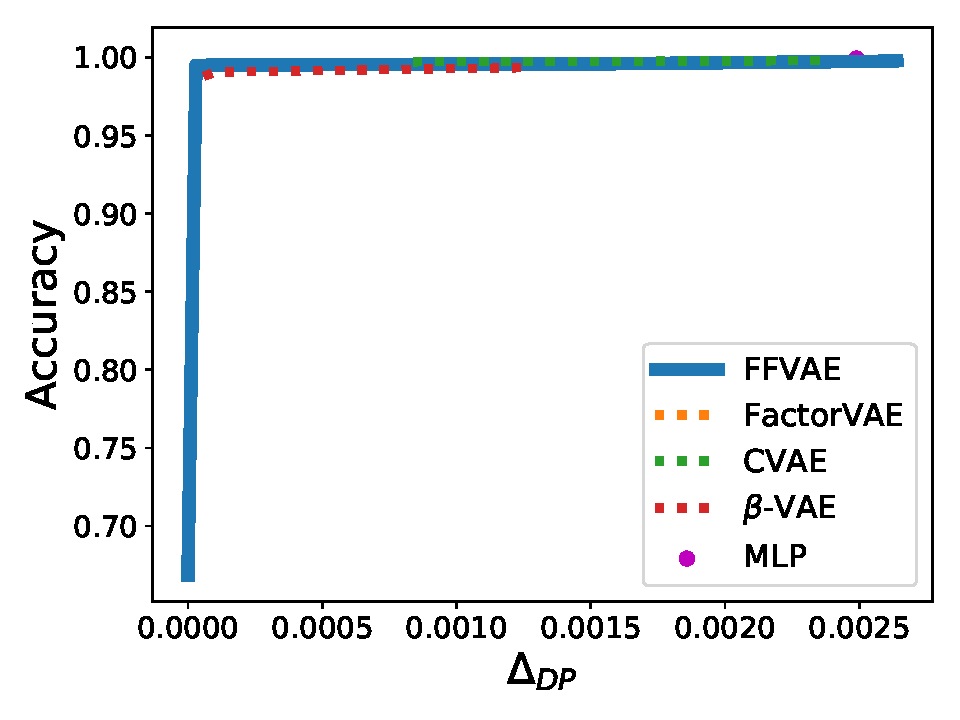
\includegraphics[width=\textwidth]{attr_fn_2_label_fn_4.pdf}
\caption{$a$ = Scale}
\label{fig:dsprites-pareto-a2-y4}
\end{subfigure}
%
\hfill
%
\begin{subfigure}[t]{\figWidth}
% \centering
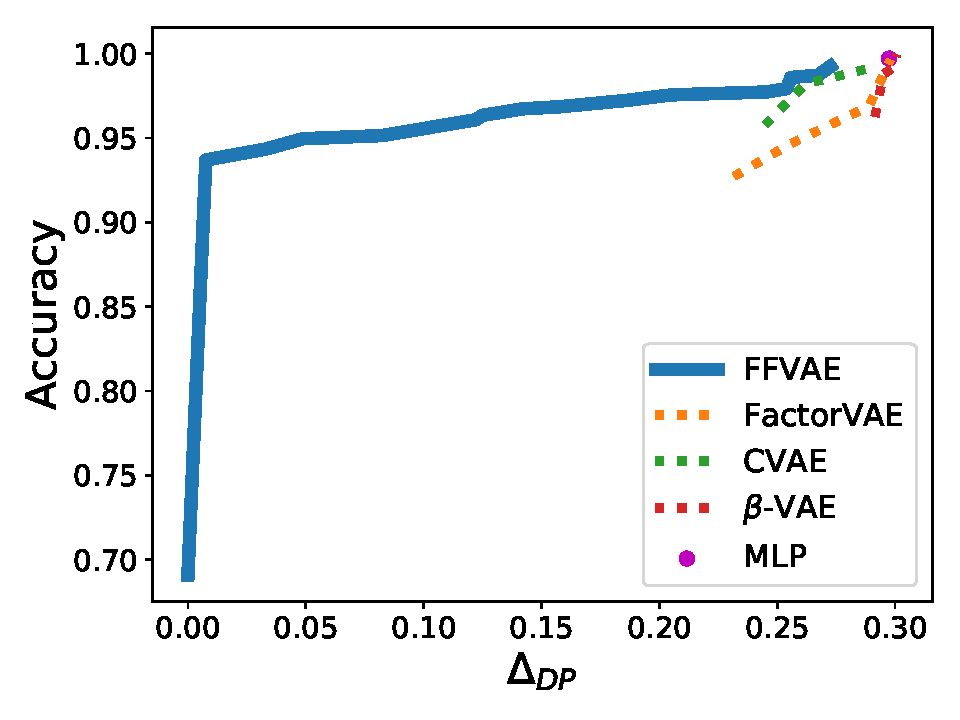
\includegraphics[width=\textwidth]{attr_fn_1_label_fn_4.pdf}
\caption{$a$ = Shape}
\label{fig:dsprites-pareto-a1-y4}
\end{subfigure}
%
\hfill
%
\begin{subfigure}[t]{\figWidth}
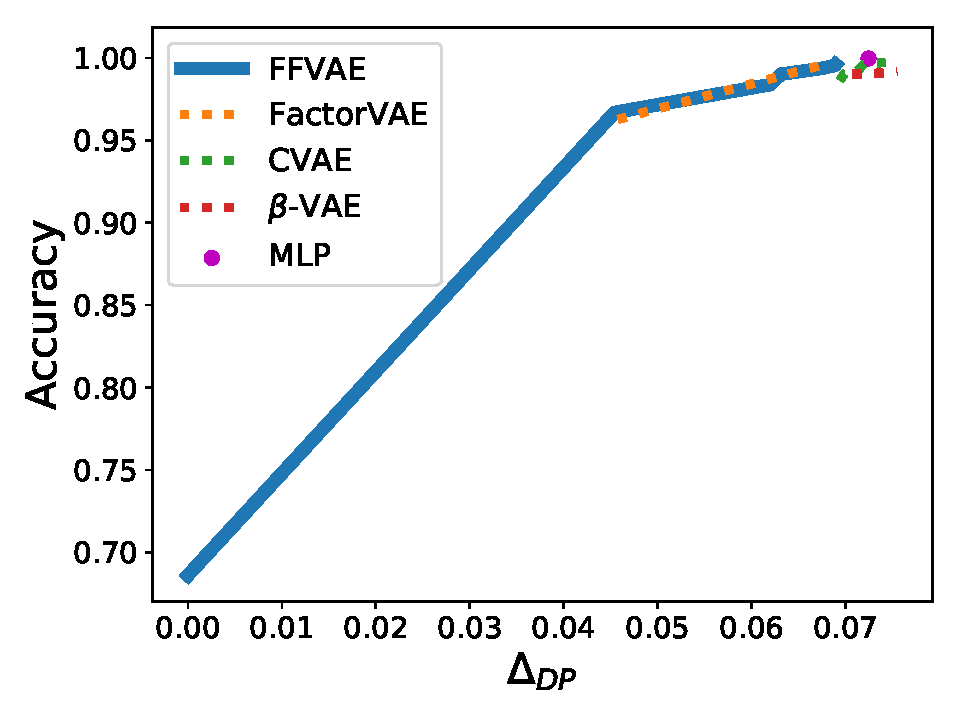
\includegraphics[width=\textwidth]{attr_fn_1_AND_attr_fn_2_label_fn_4.pdf}    
\caption{$a$ = Shape $\wedge$ Scale}
\label{fig:dsprites-pareto-a1and2-y4}
\end{subfigure}
%
\hfill
%
\begin{subfigure}[t]{\figWidth}
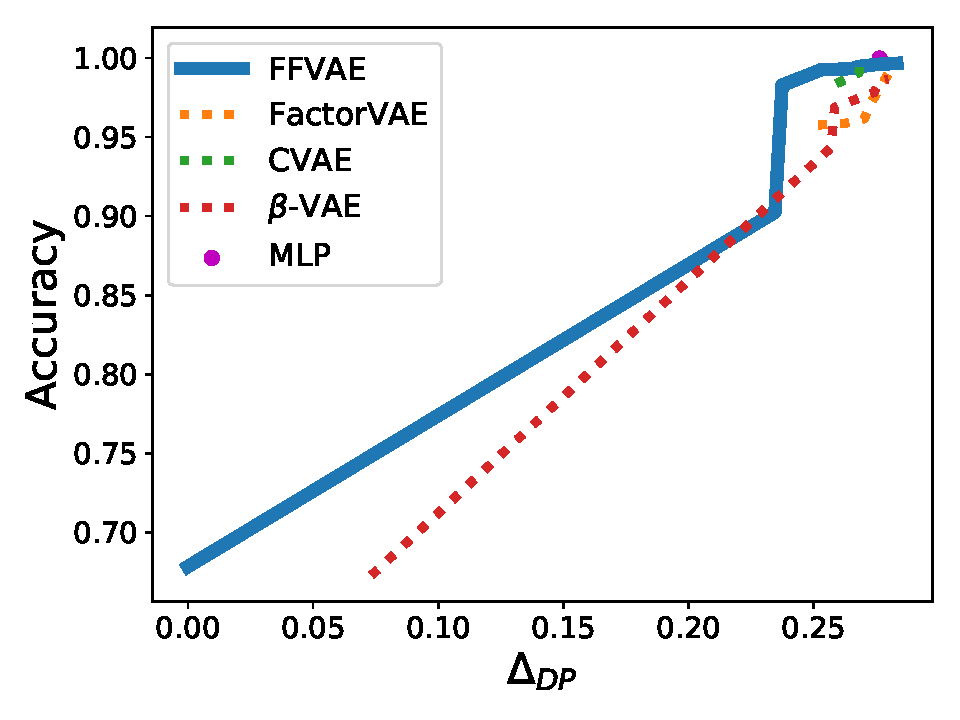
\includegraphics[width=\textwidth]{attr_fn_1_OR_attr_fn_2_label_fn_4.pdf}
\caption{$a$ = Shape $\vee$ Scale}
\label{fig:dsprites-pareto-a1or2-y4}
\end{subfigure}

\caption{
    Fairness-accuracy tradeoff curves, DSpritesUnfair dataset.
    We sweep a range of hyperparameters for each model and report Pareto fronts.
    Optimal point is the top left hand corner --- this represents perfect accuracy and fairness.
    MLP is a baseline classifier trained directly on the input data.
    For each model, encoder outputs are modified to remove information about $a$.
    $y$ = XPosition for each plot.
    }
    \label{fig:dsprites-pareto}
% \end{center}
% \vskip -0.2in
\end{figure*}

\paragraph{DSpritesUnfair Dataset}
\begin{figure}[ht!]
\centering
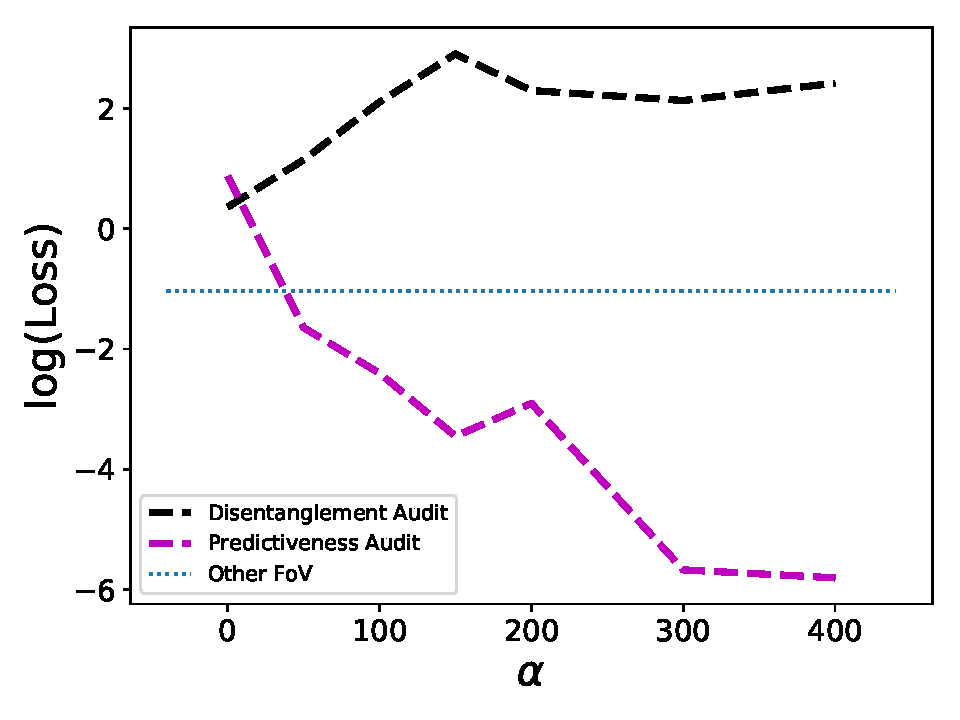
\includegraphics[width=0.4\textwidth]{dsprites_biased_val_logloss_removed_and_clf_bybetasens_a1.pdf}
\vspace{-0.2cm}
\caption{
    Black and pink dashed lines respectively show FFVAE disentanglement audit (the higher the better) and predictiveness audit (the lower the better) as a function of $\alpha$.
    These audits use $A_i$=Shape (see text for details).
    The blue line is a reference value---the log loss of a classifier that predicts $A_i$ from the other 5 DSprites factors of variation (FoV) alone, ignoring the image---representing the amount of information about $A_i$ inherent in the data.
    }
    \label{fig:dsprites-audit}
% \end{center}
% \vskip -0.2in
\end{figure}

The DSprites dataset\footnote{\scriptsize \url{https://github.com/deepmind/dsprites-dataset}} contains $64 \times 64$-pixel images of white shapes against a black background, and was designed to evaluate whether learned representations have disentangled sources of variation.
The original dataset has several categorical factors of variation---Scale, Orientation, XPosition, YPosition---that combine to create $700,000$ unique images.
We binarize the factors of variation to derive sensitive attributes and labels, so that many images now share any given attribute/label combination (See Appendix \ref{sec:dsprites-generation} for details).
In the original DSprites dataset, the factors of variation are sampled uniformly.
However, in fairness problems, we are often concerned with correlations between attributes and the labels we are trying to predict (otherwise, achieving low $\Delta_{DP}$ is aligned with standard classification objectives).
Hence, we sampled an ``unfair'' version of this data (DSpritesUnfair) with correlated factors of variation; in particular Shape and XPosition correlate positively.
Then a non-trivial fair classification task would be, for instance, learning to predict shape without discriminating against inputs from the left side of the image.

\paragraph{Baselines}
To test the utility of our predictiveness prior, we compare our model to $\beta$-VAE (VAE with a coefficient $\beta \geq 1$ on the KL term) and FactorVAE, which have disentanglement priors but no predictiveness prior.
We can also think of these as FFVAE with $\alpha = 0$.
To test the utility of our disentanglement prior, we also compare against a version of our model with $\gamma = 0$, denoted CVAE.
This is similar to the class-conditional VAE \citep{kingma2014semi}, with sensitive attributes as labels --- this model encourages predictiveness but no disentanglement.

\paragraph{Fair Classification}
We perform the fair classification audit using several group/subgroup definitions for models trained on DSpritesUnfair (see Appendix \ref{sec:dsprites-training-details} for training details), and report fairness-accuracy tradeoff curves in Fig. \ref{fig:dsprites-pareto}.
In these experiments, we used Shape and Scale as our sensitive attributes during encoder training.
We perform the fair classification audit by training an MLP to predict $y=$``XPosition''% (horizontal position of the shape), 
---which was not used in the representation learning phase---given the modified encoder outputs, and repeat for several sensitive groups and subgroups.
We modify the encoder outputs as follows:
When our sensitive attribute is $a_i$ we remove the associated dimension $b_i$ from $[z,b]$; when the attribute is a conjunction of $a_i$ and $a_j$, we remove both $b_i$ and $b_j$.
For the baselines, we simply remove the latent dimension which is most correlated with $a_i$, or the two most correlated dimensions with the conjunction.
We sweep a range of hyperparameters to produce the fairness-accuracy tradeoff curve for each model.
In Fig. \ref{fig:dsprites-pareto}, we show the ``Pareto front'' of these models: points in ($\Delta_{DP}$, accuracy)-space for which no other point is better along both dimensions.
The optimal result is the top left hand corner (perfect accuracy and $\Delta_{DP} = 0$).

Since we have a 2-D sensitive input space, we show results for four different sensitive attributes derived from these dimensions: $\{a=\text{``Shape''}, a=\text{``Scale''}, a=\text{``Shape''}\vee\text{``Scale''}, a=\text{``Shape''}\wedge\text{``Scale''}\}$.
Recall that Shape and XPosition correlate in the DSpritesUnfair dataset.
Therefore, for sensitive attributes that involve Shape, we expect to see an improvement in $\Delta_{DP}$.
For sensitive attributes that do not involve Shape, we expect that our method does not hurt performance at all --- since the attributes are uncorrelated in the data, the optimal predictive solution also has $\Delta_{DP} = 0$.

When group membership $a$ is uncorrelated with label $y$ (Fig. \ref{fig:dsprites-pareto-a2-y4}), all models achieve high accuracy and low $\Delta_{DP}$ ($a$ and $y$ successfully disentangled).
When $a$ correlates with $y$ by design (Fig. \ref{fig:dsprites-pareto-a1-y4}), we see the clearest improvement of the FFVAE over the baselines, with an almost complete reduction in $\Delta_{DP}$ and very little accuracy loss.
The baseline models are all unable to improve $\Delta_{DP}$ by more than about 0.05, indicating that they have not effectively disentangled the sensitive information from the label.
In Figs. \ref{fig:dsprites-pareto-a1and2-y4} and \ref{fig:dsprites-pareto-a1or2-y4}, we examine conjunctions of sensitive attributes, assessing FFVAE's ability to flexibly provide multi-attribute fair representations.
Here FFVAE exceeds or matches the baselines accuracy-at-a-given-$\Delta_{DP}$ almost everywhere;
by disentangling information from multiple sensitive attributes, FFVAE enables flexibly fair downstream classification.

\paragraph{Disentanglement and Predictiveness}
Fig. \ref{fig:dsprites-audit} shows the FFVAE disentanglement and predictiveness audits (see above for description of this procedure).
This result aggregates audits across all FFVAE models trained in the setting from Figure \ref{fig:dsprites-pareto-a1-y4}.
The classifier loss is cross-entropy, which is a lower bound on the mutual information between the input and target of the classifier.
We observe that increasing $\alpha$ helps both predictiveness and disentanglement in this scenario.
In the disentanglement audit, larger $\alpha$ makes predicting the sensitive attribute from the modified representation (with $b_i$ removed) more difficult.
The horizontal dotted line shows the log loss of a classifier that predicts $a_i$ from the other DSprites factors of variation (including labels not available to FFVAE); this baseline reflects the correlation inherent in the data.
We see that when $\alpha = 0$ (i.e. FactorVAE), it is slightly more difficult than this baseline to predict the sensitive attribute.
This is due to the disentanglement prior.
However, increasing $\alpha > 0$ increases disentanglement benefits in FFVAE beyond what is present in FactorVAE.
This shows that encouraging predictive structure can help disentanglement through isolating each attribute's information in particular latent dimensions.
Additionally, increasing $\alpha$ improves predictiveness, as expected from the objective formulation.
We further evaluate the disentanglement properties of our model in Appendix \ref{sec:mig} using the Mutual Information Gap metric \cite{chen2018isolating}.

\subsection{Communities \& Crime} \label{sec:communities}
\paragraph{Dataset}
Communities \& Crime\footnote{\scriptsize \url{http://archive.ics.uci.edu/ml/datasets/communities+and+crime}} is a tabular UCI dataset containing neighborhood-level population statistics. 
120 such statistics are recorded for each of the $1,994$ neighborhoods. 
Several attributes encode demographic information that may be protected. We chose three as sensitive: racePctBlack (\% neighborhood population which is Black), blackPerCap (avg per capita income of Black residents), and pctNotSpeakEnglWell (\% neighborhood population that does not speak English well). 
We follow the same train/eval procedure as with DSpritesUnfair - we train FFVAE with the sensitive attributes and evaluate using naive MLPs to predict a held-out label (violent crimes per capita) on held-out data.

\newcommand{\thirdFigWidth}{0.15\textwidth}

\begin{figure}[ht!]
%
% \begin{center}
% \centering
\begin{subfigure}[t]{\thirdFigWidth}
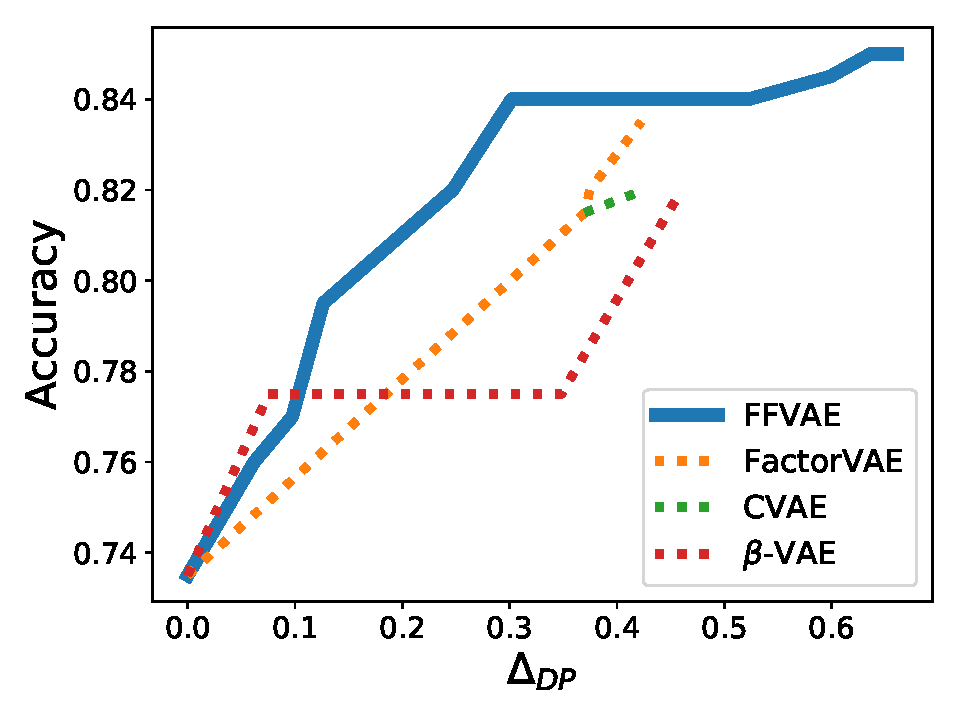
\includegraphics[width=\textwidth]{cc_attr_fn_0.pdf}
\caption{$a$ = R}
\label{fig:cc_attr_fn_0}
\end{subfigure}
%
\hfill
%
\begin{subfigure}[t]{\thirdFigWidth}
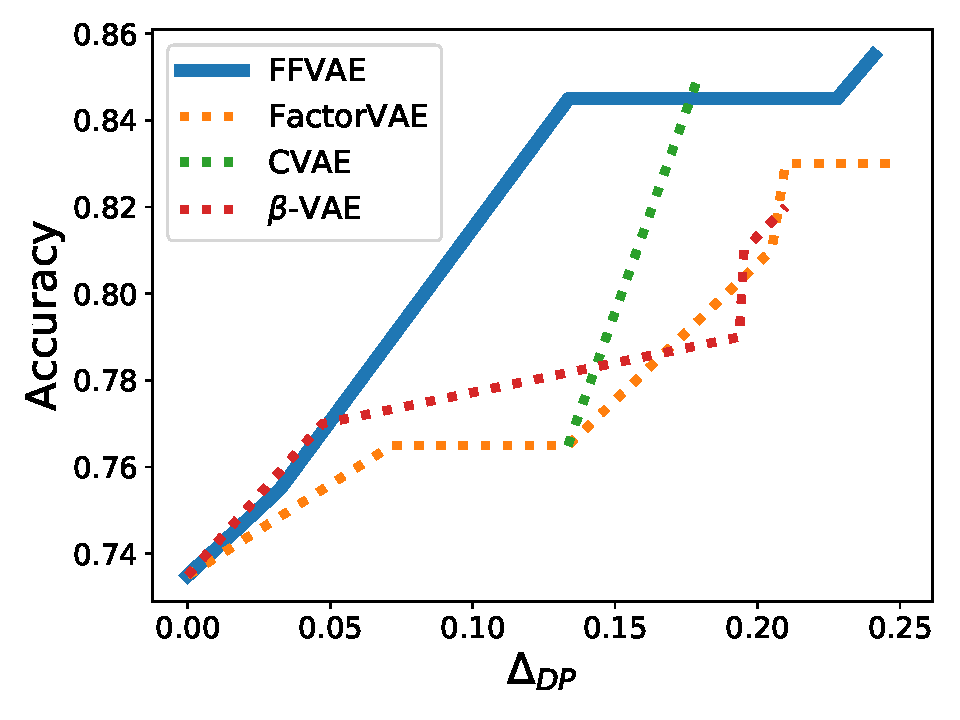
\includegraphics[width=\textwidth]{cc_attr_fn_5.pdf}
\caption{$a$ = B}
\label{fig:cc_attr_fn_5}
\end{subfigure}
%
\hfill
%
\begin{subfigure}[t]{\thirdFigWidth}
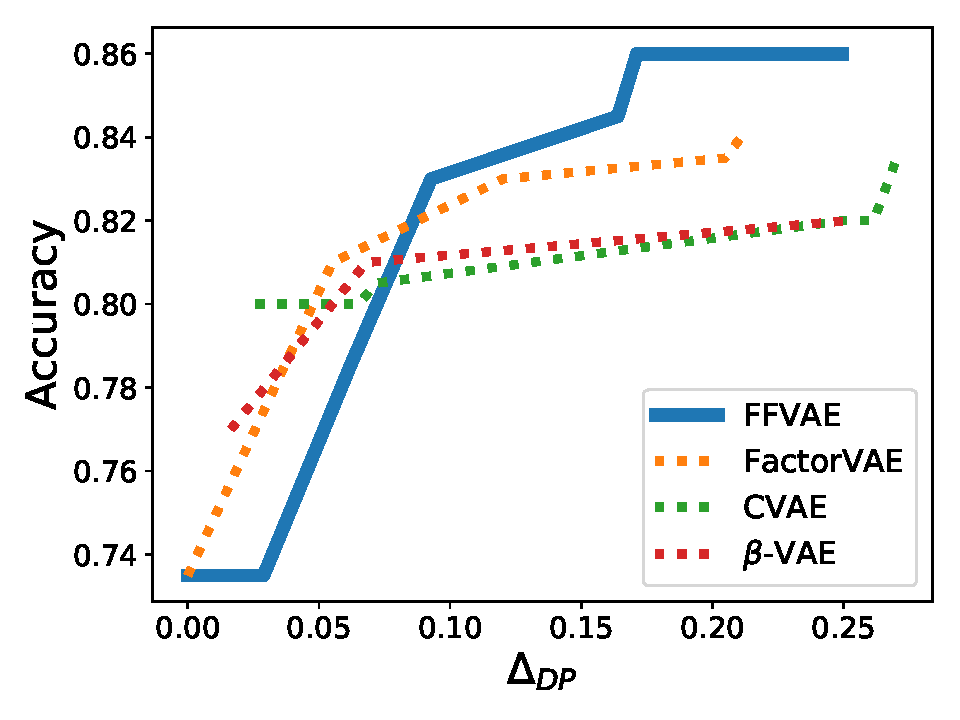
\includegraphics[width=\textwidth]{cc_attr_fn_11.pdf}
\caption{$a$ = P}
\label{fig:cc_attr_fn_11}
\end{subfigure}
%
\hfill
%
\begin{subfigure}[t]{\thirdFigWidth}
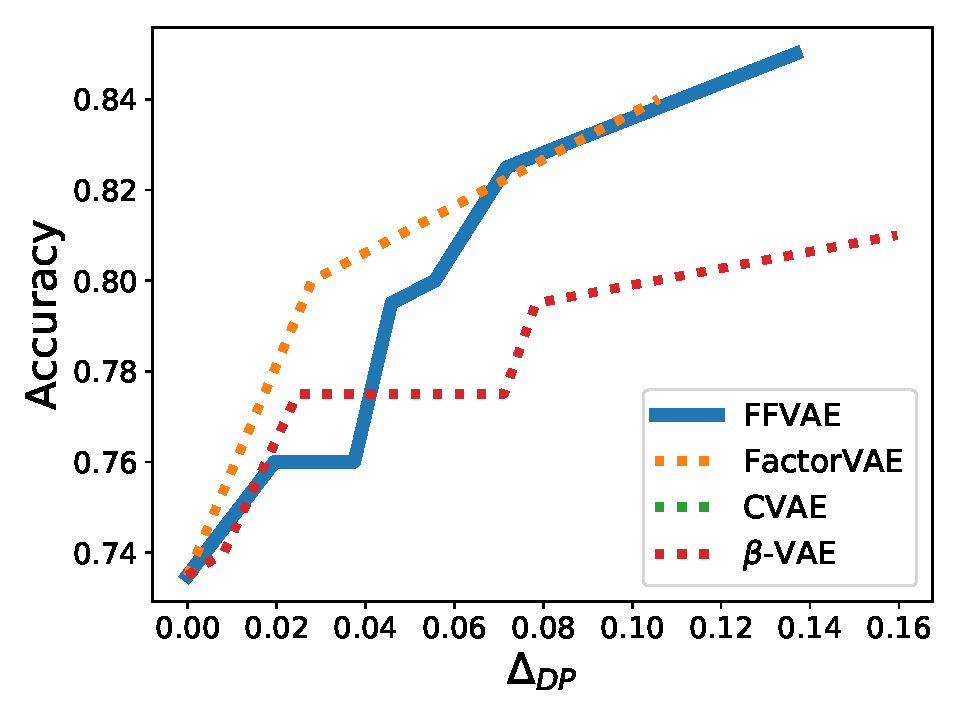
\includegraphics[width=\textwidth]{cc_attr_fn_0_OR_cc_attr_fn_5.pdf}
\caption{$a$ = R $\vee$ B}
\label{fig:cc_attr_fn_0_OR_cc_attr_fn_5}
\end{subfigure}
%
\hfill
%
\begin{subfigure}[t]{\thirdFigWidth}
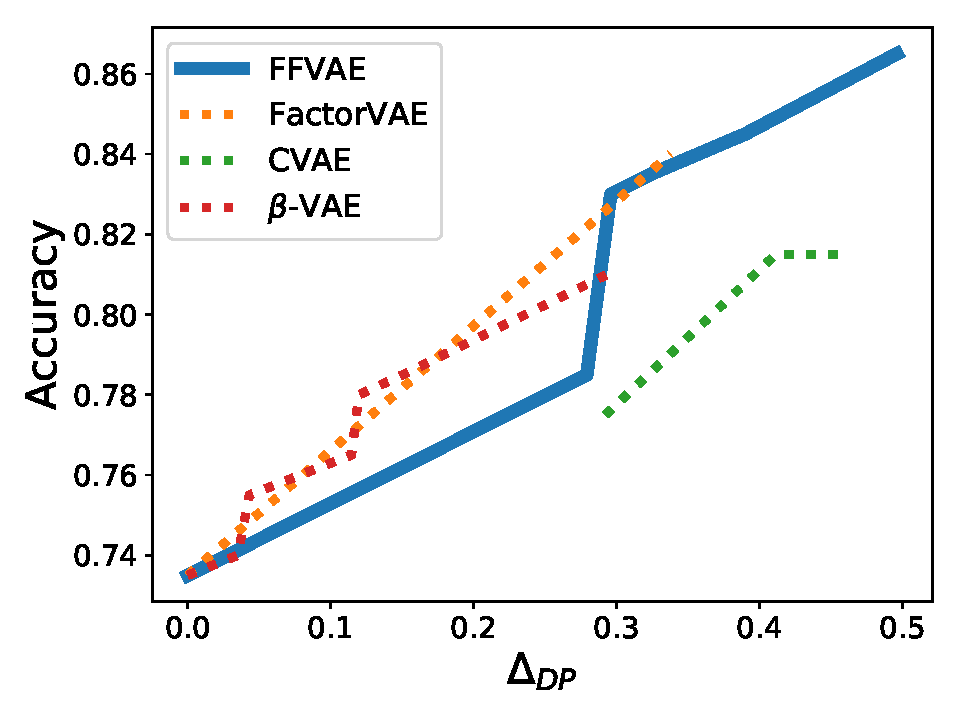
\includegraphics[width=\textwidth]{cc_attr_fn_0_OR_cc_attr_fn_11.pdf}
\caption{$a$ = R $\vee$ P}
\label{fig:cc_attr_fn_0_OR_cc_attr_fn_11}
\end{subfigure}
%
\hfill
%
\begin{subfigure}[t]{\thirdFigWidth}
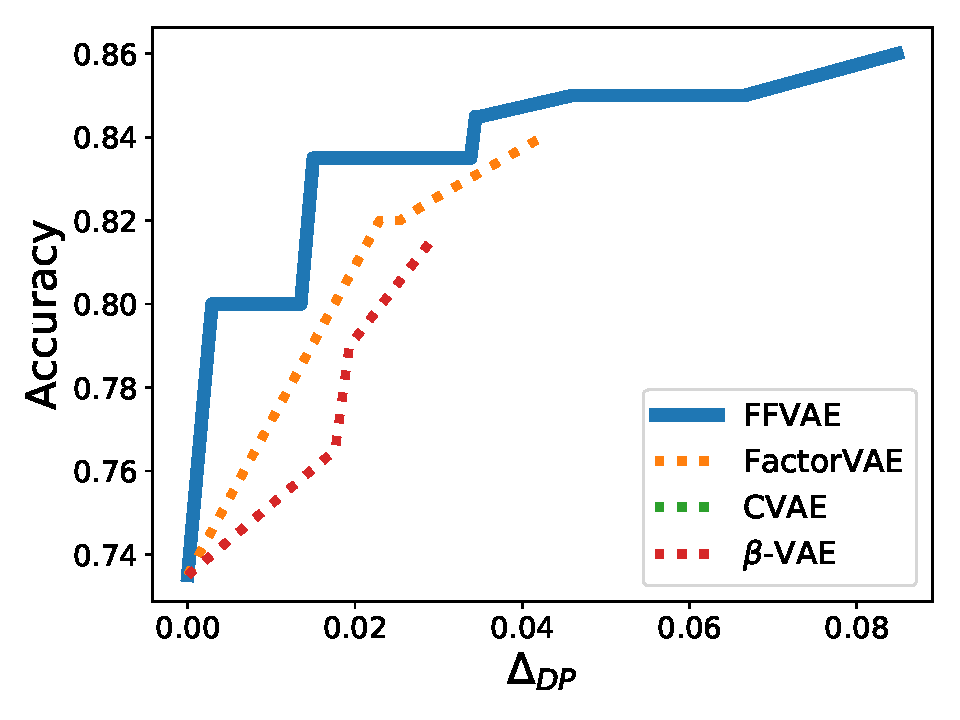
\includegraphics[width=\textwidth]{cc_attr_fn_5_OR_cc_attr_fn_11.pdf}
\caption{$a$ = B $\vee$ P}
\label{fig:cc_attr_fn_5_OR_cc_attr_fn_11}
\end{subfigure}
%
\hfill
%
\begin{subfigure}[t]{\thirdFigWidth}
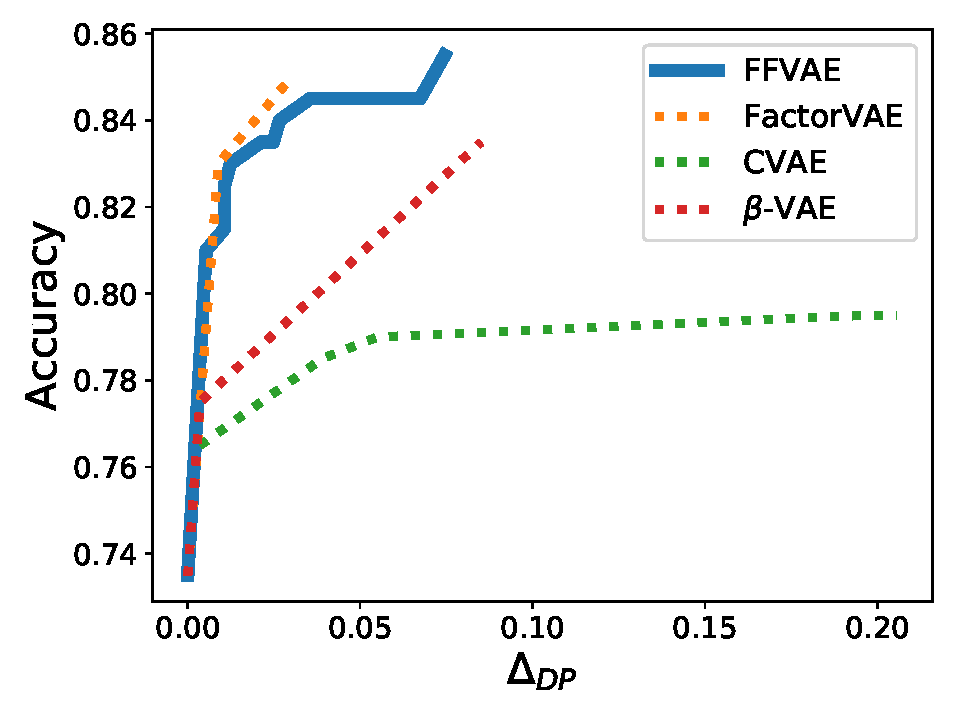
\includegraphics[width=\textwidth]{cc_attr_fn_0_AND_cc_attr_fn_5.pdf}
\caption{$a$ = R $\wedge$ B}
\label{fig:cc_attr_fn_0_AND_cc_attr_fn_5}
\end{subfigure}
%
\hfill
%
\begin{subfigure}[t]{\thirdFigWidth}
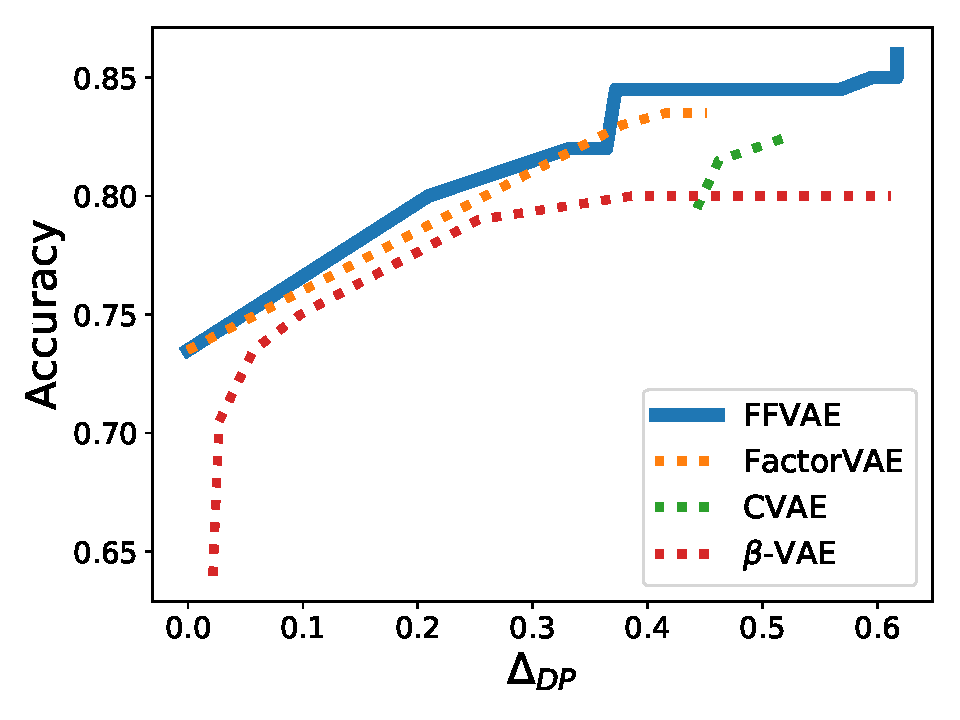
\includegraphics[width=\textwidth]{cc_attr_fn_0_AND_cc_attr_fn_11.pdf}
\caption{$a$ = R $\wedge$ P}
\label{fig:cc_attr_fn_0_AND_cc_attr_fn_11}
\end{subfigure}
%
\hfill
%
\begin{subfigure}[t]{\thirdFigWidth}
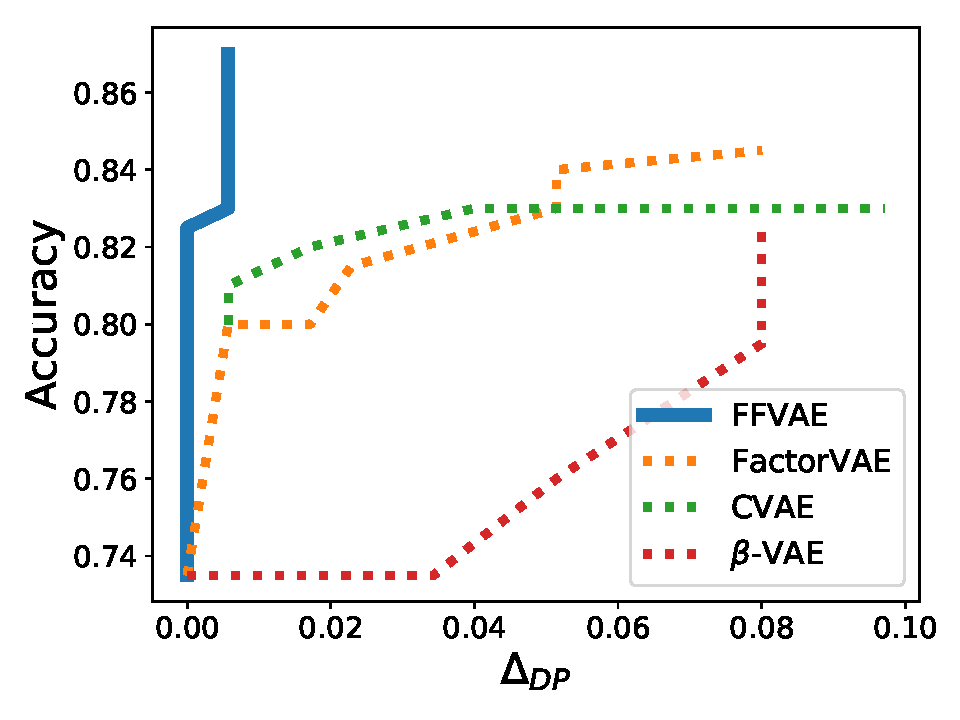
\includegraphics[width=\textwidth]{cc_attr_fn_5_AND_cc_attr_fn_11.pdf}
\caption{$a$ = B $\wedge$ P}
\label{fig:cc_attr_fn_5_AND_cc_attr_fn_11}
\end{subfigure}
%
\hfill


\caption{
    Communities \& Crime subgroup fairness-accuracy tradeoffs.
    Sensitive attributes: racePctBlack (R), blackPerCapIncome (B), and pctNotSpeakEnglWell (P).
    $y$ = violentCrimesPerCaptia. 
    }
    \label{fig:comcrime-pareto}
% \end{center}
% \vskip -0.2in
\end{figure}


\paragraph{Fair Classification}
This dataset presents a more difficult disentanglement problem than DSpritesUnfair.
The three sensitive attributes we chose in Communities and Crime were somewhat correlated with each other, a natural artefact of using real (rather than simulated) data.
We note that in general, the disentanglement literature does not provide much guidance in terms of disentangling correlated attributes.
Despite this obstacle, FFVAE performed reasonably well in the fair classification audit (Fig. \ref{fig:comcrime-pareto}).
It achieved higher accuracy than the baselines in general, likely due to its ability to incorporate side information from $a$ during training.
Among the baselines, FactorVAE tended perform best, suggesting achieving a factorized aggregate posterior helps with fair classification.
While our method does not outperform the baselines on each conjunction, its relatively strong performance on a difficult, tabular dataset shows the promise of using disentanglement priors in designing robust subgroup-fair machine learning models.

\subsection{Celebrity Faces} \label{sec:celeba}

%\newcommand{\thirdFigWidth}{0.15\textwidth}

\begin{figure}[ht!]
%
% \begin{center}
% \centering
\begin{subfigure}[t]{\thirdFigWidth}
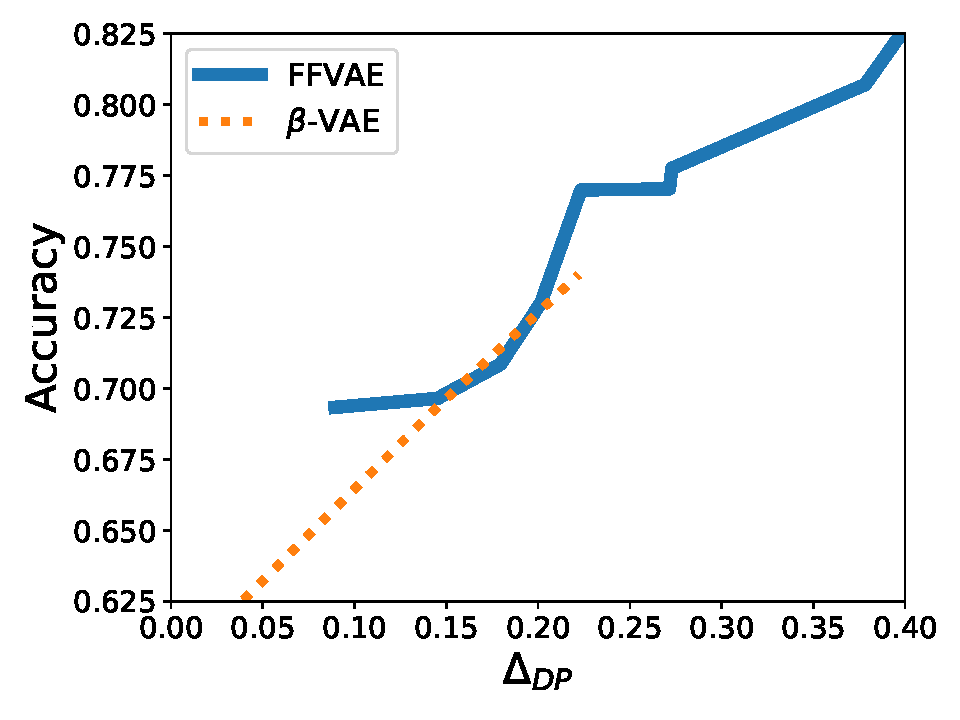
\includegraphics[width=\textwidth]{predict_C.pdf}
\caption{$a$ = C}
\label{fig:predict_C}
\end{subfigure}
%
\hfill
%
\begin{subfigure}[t]{\thirdFigWidth}
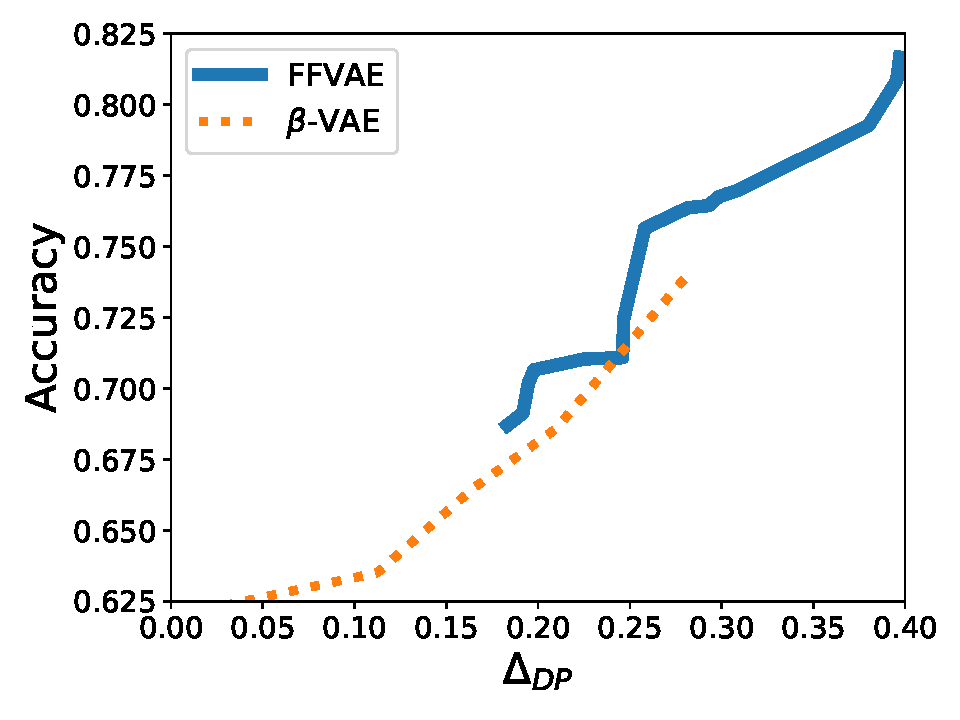
\includegraphics[width=\textwidth]{predict_E.pdf}
\caption{$a$ = E}
\label{fig:predict_E}
\end{subfigure}
%
\hfill
%
\begin{subfigure}[t]{\thirdFigWidth}
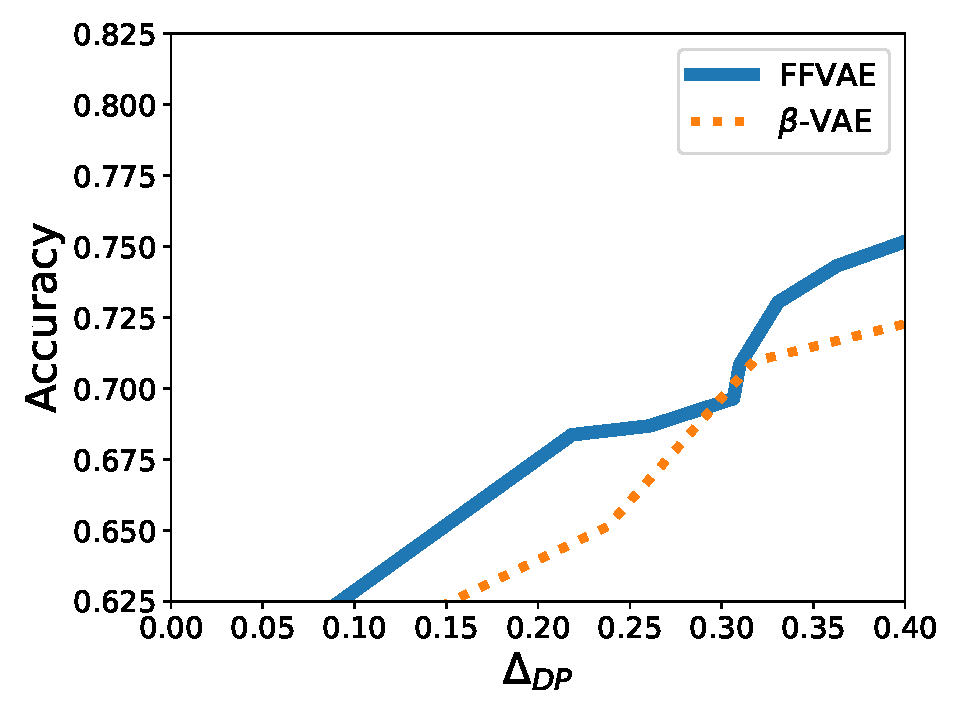
\includegraphics[width=\textwidth]{predict_M.pdf}
\caption{$a$ = M}
\label{fig:predict_M}
\end{subfigure}
%
\hfill
%
\begin{subfigure}[t]{\thirdFigWidth}
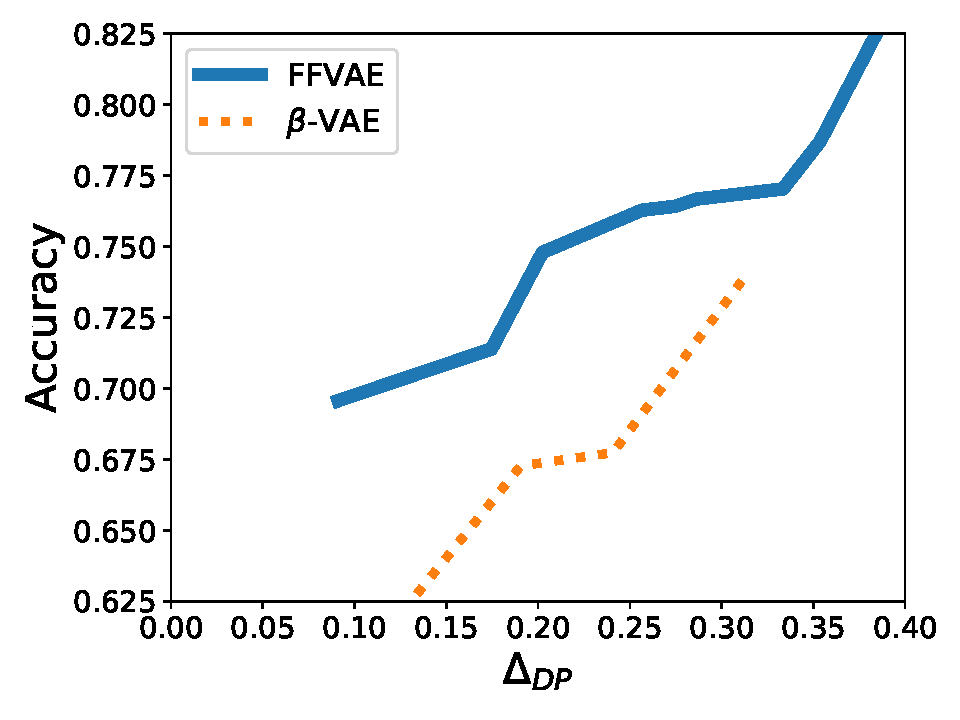
\includegraphics[width=\textwidth]{predict_C-AND-E.pdf}
\caption{$a$ = C $\wedge$ E}
\label{fig:predict_C-AND-E}
\end{subfigure}
%
\hfill
%
\begin{subfigure}[t]{\thirdFigWidth}
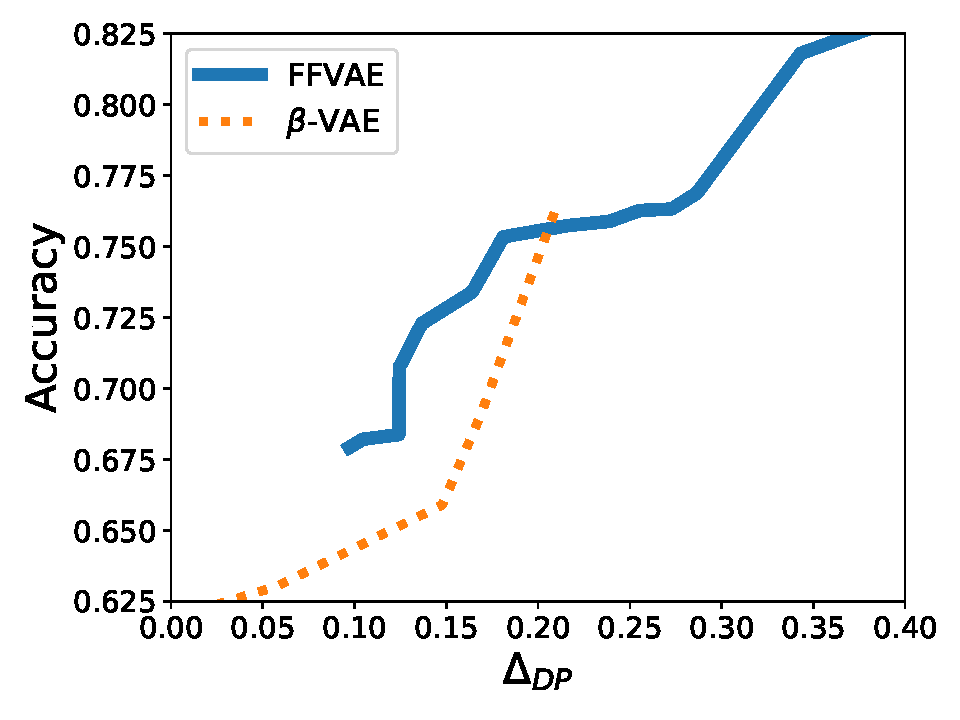
\includegraphics[width=\textwidth]{predict_C-AND-NOT-E.pdf}
\caption{$a$ = C $\wedge \neg$ E}
\label{fig:predict_C-AND-NOT-E}
\end{subfigure}
%
\hfill
%
\begin{subfigure}[t]{\thirdFigWidth}
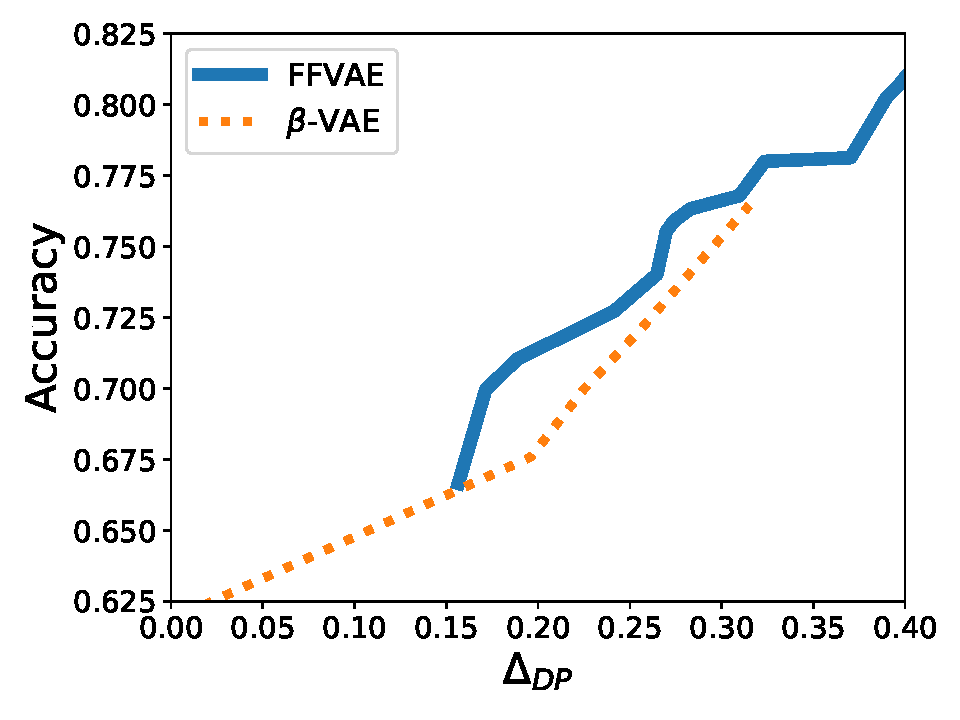
\includegraphics[width=\textwidth]{predict_NOT-C-AND-E.pdf}
\caption{$a$ = $\neg$ C $\wedge$ E}
\label{fig:predict_NOT-C-AND-E}
\end{subfigure}
%
\hfill
%
\begin{subfigure}[t]{\thirdFigWidth}
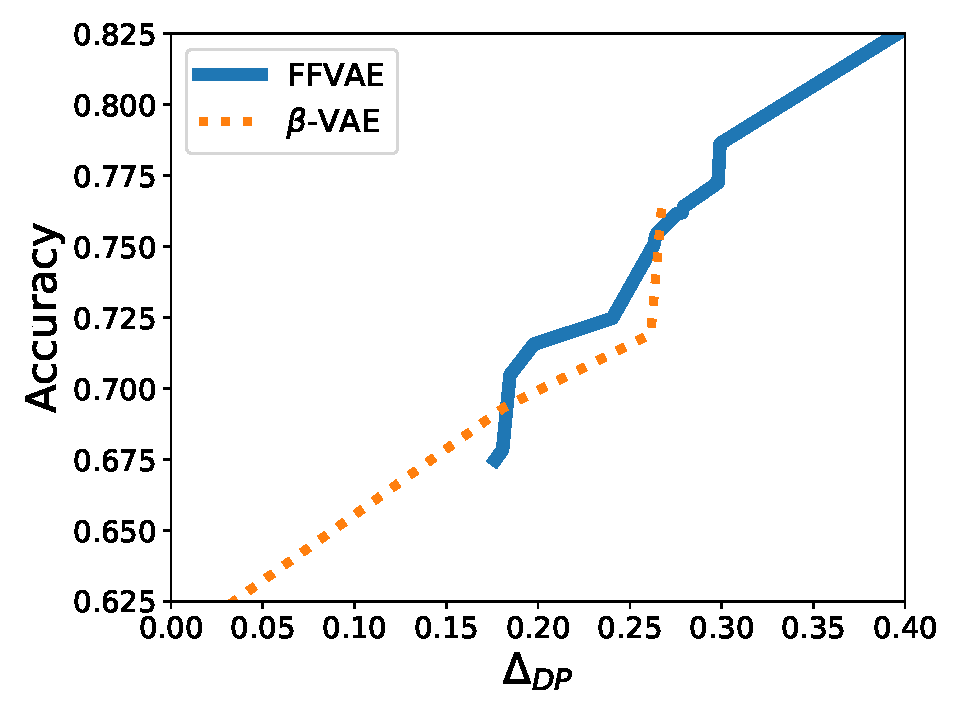
\includegraphics[width=\textwidth]{predict_NOT-C-AND-NOT-E.pdf}
\caption{$a$ = $\neg$ C $\wedge \neg$ E}
\label{fig:predict_NOT-C-AND-NOT-E}
\end{subfigure}
%
\hfill
%
\begin{subfigure}[t]{\thirdFigWidth}
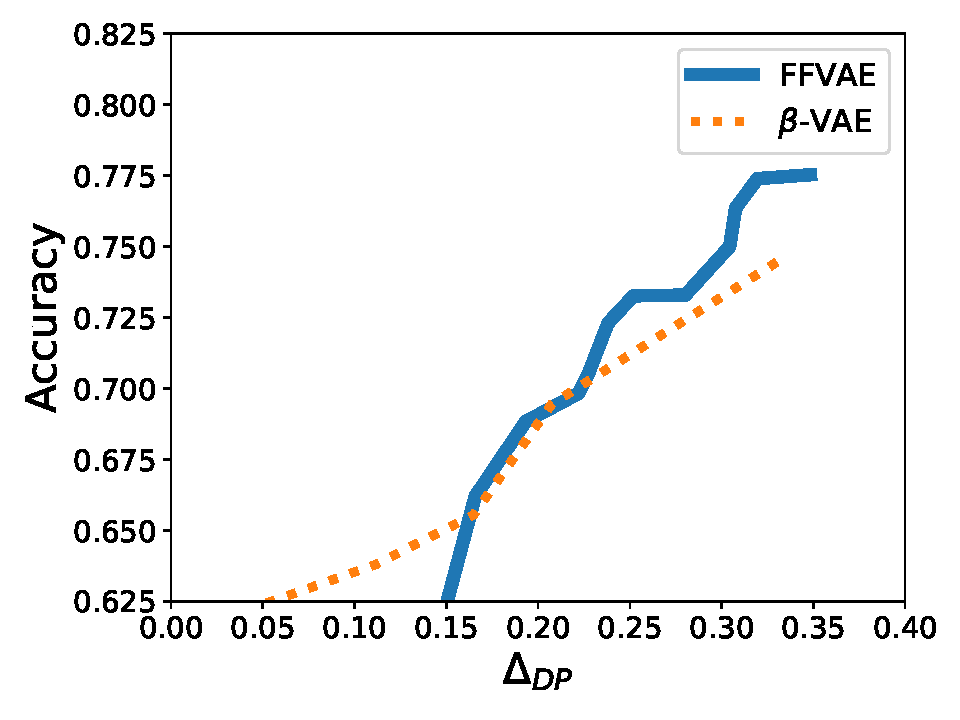
\includegraphics[width=\textwidth]{predict_C-AND-M.pdf}
\caption{$a$ = C $\wedge$ M}
\label{fig:predict_C-AND-M}
\end{subfigure}
%
\hfill
%
\begin{subfigure}[t]{\thirdFigWidth}
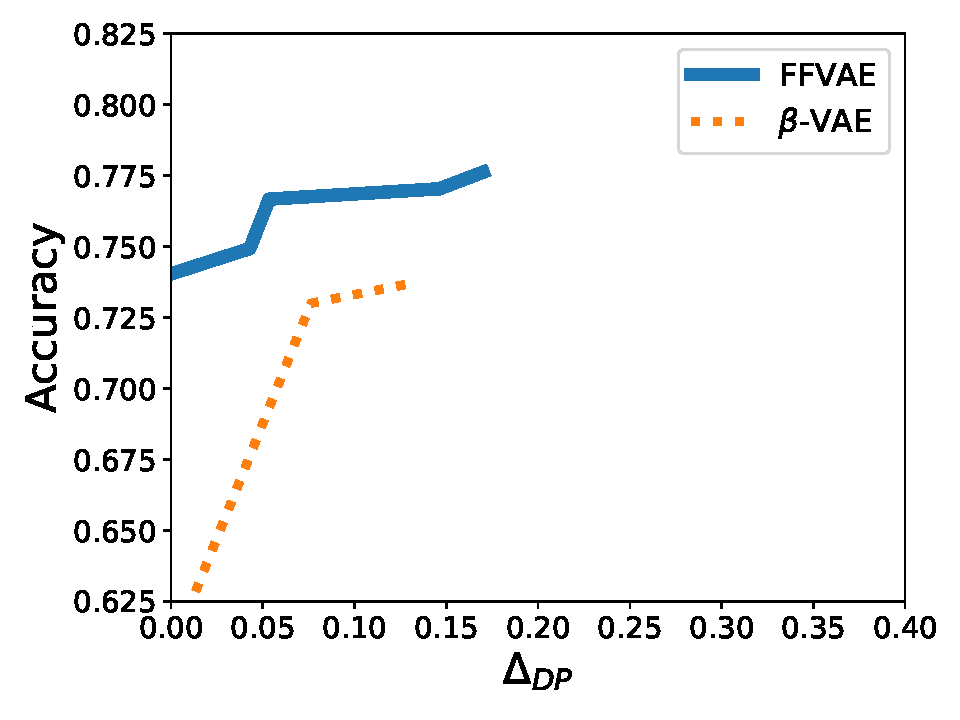
\includegraphics[width=\textwidth]{predict_C-AND-NOT-M.pdf}
\caption{$a$ = C $\wedge \neg$ M}
\label{fig:predict_C-AND-NOT-M}
\end{subfigure}
%
\hfill
%
\begin{subfigure}[t]{\thirdFigWidth}
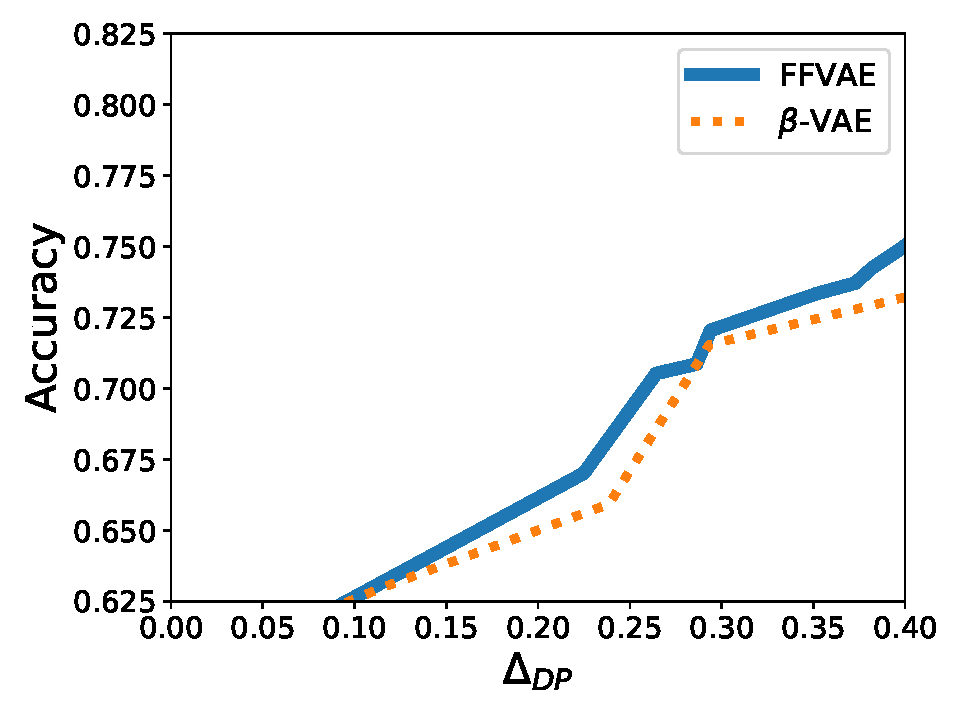
\includegraphics[width=\textwidth]{predict_NOT-C-AND-M.pdf}
\caption{$a$ = $\neg$ C $\wedge$ M}
\label{fig:predict_NOT-C-AND-M}
\end{subfigure}
%
\hfill
%
\begin{subfigure}[t]{\thirdFigWidth}
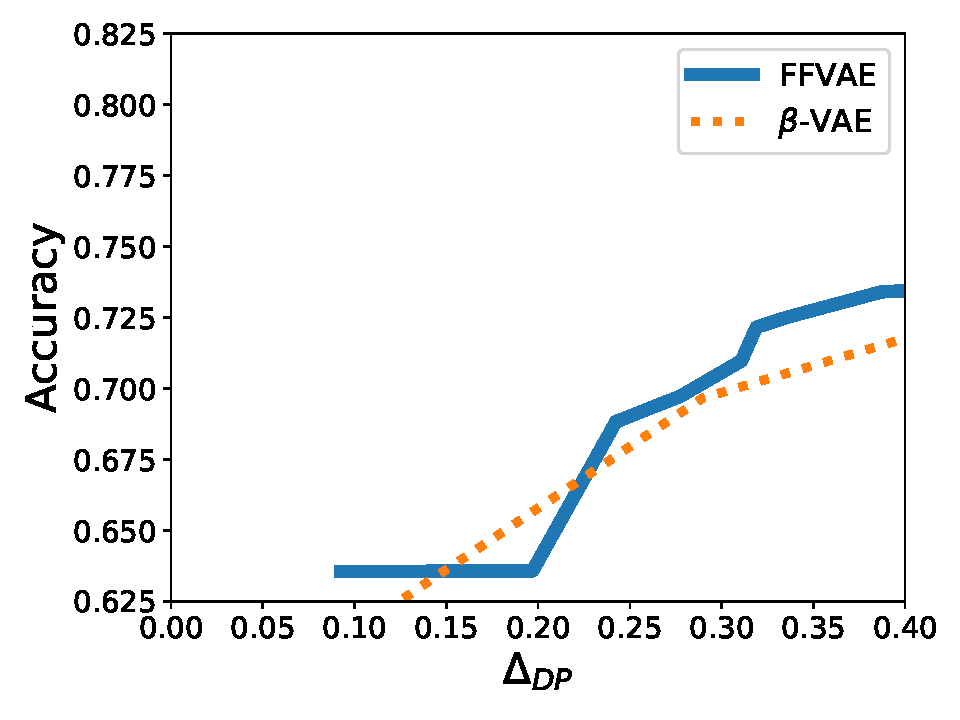
\includegraphics[width=\textwidth]{predict_NOT-C-AND-NOT-M.pdf}
\caption{$a$ = $\neg$ C $\wedge \neg$ M}
\label{fig:predict_NOT-C-AND-NOT-M}
\end{subfigure}
%
\hfill
%
\begin{subfigure}[t]{\thirdFigWidth}
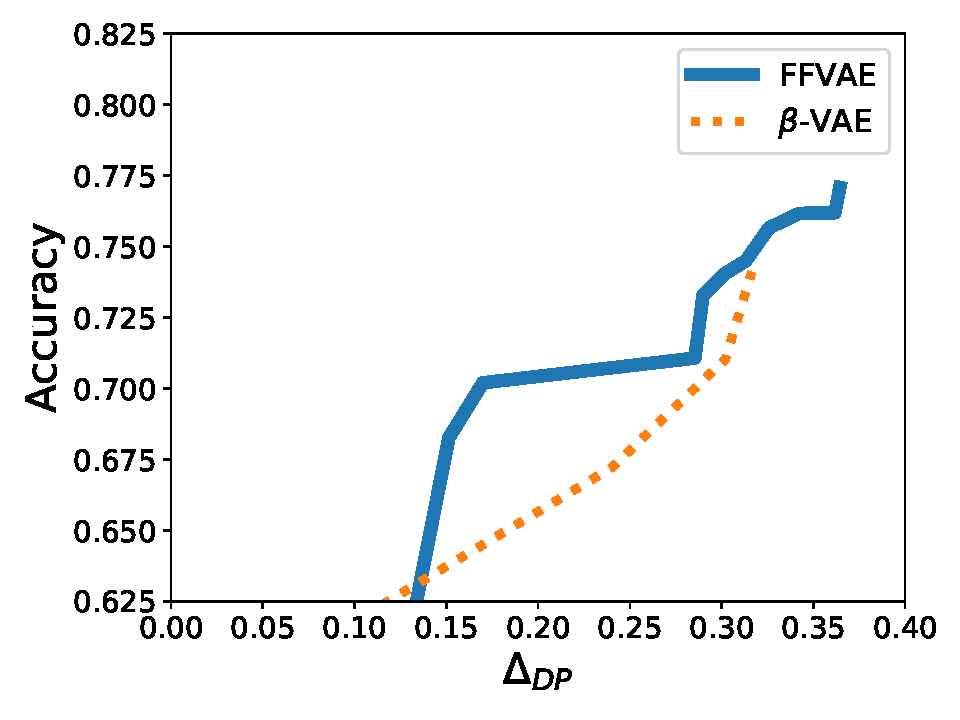
\includegraphics[width=\textwidth]{predict_E-AND-M.pdf}
\caption{$a$ = $\neg$ E $\wedge$ M}
\label{fig:predict_E-AND-M}
\end{subfigure}
%
\hfill

%
\begin{subfigure}[t]{\thirdFigWidth}
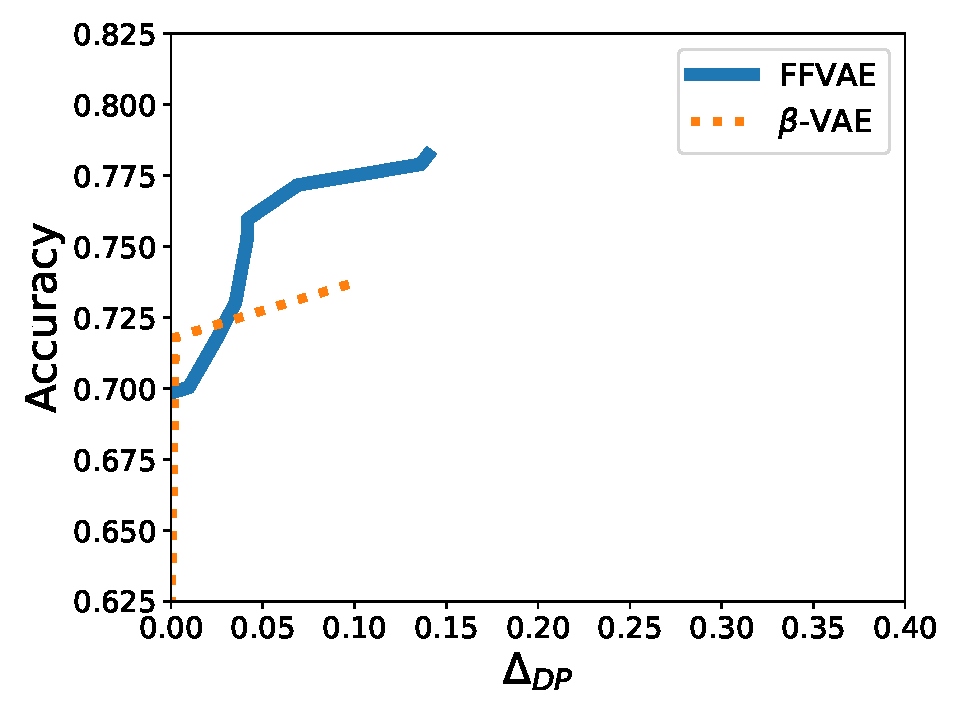
\includegraphics[width=\textwidth]{predict_E-AND-NOT-M.pdf}
\caption{$a$ = E $\wedge \neg$ M}
\label{fig:predict_E-AND-NOT-M}
\end{subfigure}
%
\hfill
%
\begin{subfigure}[t]{\thirdFigWidth}
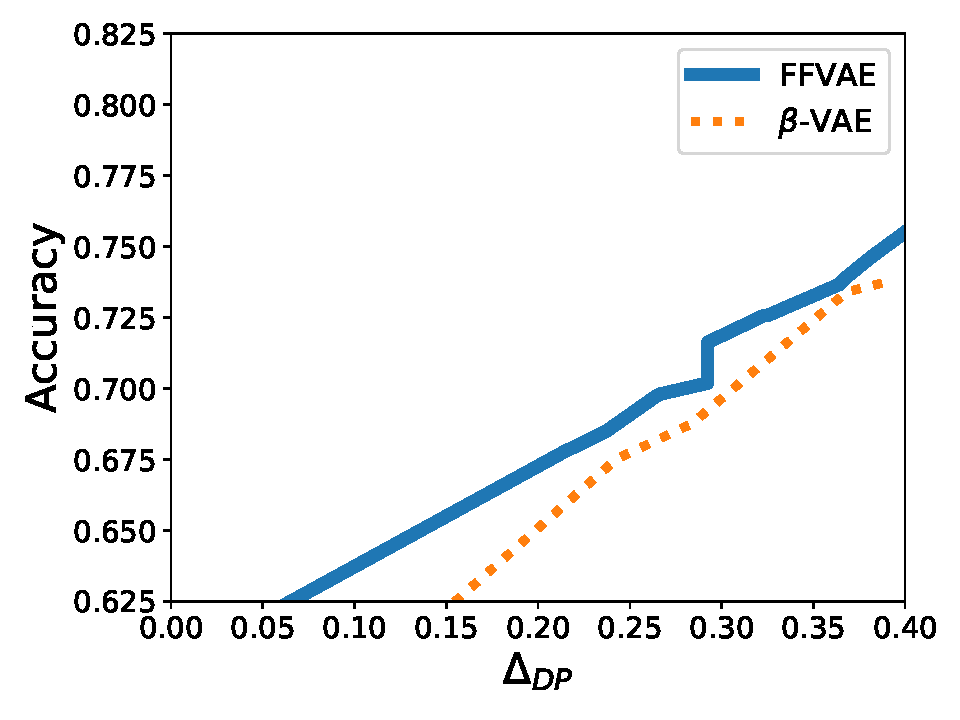
\includegraphics[width=\textwidth]{predict_NOT-E-AND-M.pdf}
\caption{$a$ = $\neg$ E $\wedge$ M}
\label{fig:predict_NOT-E-AND-M}
\end{subfigure}
%
\hfill
%
\begin{subfigure}[t]{\thirdFigWidth}
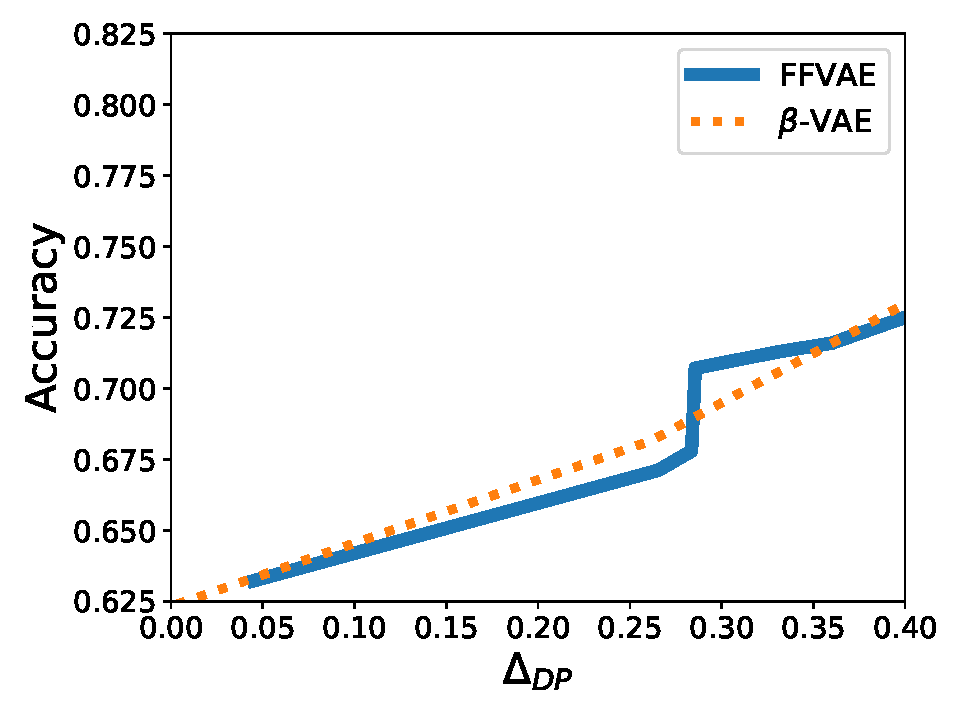
\includegraphics[width=\textwidth]{predict_NOT-E-AND-NOT-M.pdf}
\caption{$a$ = $\neg$ E $\wedge \neg$ M}
\label{fig:predict_NOT-E-AND-NOT-M}
\end{subfigure}
%
\hfill

\caption{
    Celeb-A subgroup fair classification results.
    Sensitive attributes: Chubby (C), Eyeglasses (E), and Male (M).
    $y$ = HeavyMakeup. 
    }
    \label{fig:celeba-pareto}
% \end{center}
% \vskip -0.2in
\end{figure}


\paragraph{Dataset}
The CelebA\footnote{\scriptsize \url{http://mmlab.ie.cuhk.edu.hk/projects/CelebA.html}} dataset contains over $200,000$ images of celebrity faces.
Each image is associated with 40 human-labeled binary attributes (OvalFace, HeavyMakeup, etc.).
We chose three attributes, Chubby, Eyeglasses, and Male as sensitive attributes\footnote{
We chose these attributes because they co-vary relatively weakly with each other (compared with other attribute triplets), but strongly with other attributes.
Nevertheless the rich correlation structure amongst all attributes makes this a challenging fairness dataset; it is difficult to achieve high accuracy and low $\Delta_{DP}$.
}, and report fair classification results on 3 groups and 12 two-attribute-conjunction subgroups only (for brevity we omit three-attribute conjunctions).
To our knowledge this is the first exploration of fair representation learning algorithms on the Celeb-A dataset.
As in the previous sections we train the encoders on the train set, then evaluate performance of MLP classifiers trained on the encoded test set.

\paragraph{Fair Classification}

We follow the fair classification audit procedure described above, where the held-out label HeavyMakeup---which was not used at encoder train time---is predicted by an MLP from the encoder representations.
When training the MLPs we take a fresh encoder sample for each minibatch (statically encoding the dataset with one encoder sample per image induced overfitting).
We found that training the MLPs on encoder means (rather than samples) increased accuracy but at the cost of very unfavorable $\Delta_{DP}$.
We also found that FactorVAE-style adversarial training does not scale well to this high-dimensional problem, so we instead optimize Equation \ref{eq:ffvae} using the biased estimator from \citet{chen2018isolating}.
Figure \ref{fig:celeba-pareto} shows Pareto fronts that capture the fairness-accuracy tradeoff for FFVAE and $\beta$-VAE.

While neither method dominates in this challenging setting, FFVAE achieves a favorable fairness-accuracy tradeoff across many of subgroups.
We believe that using sensitive attributes as side information gives FFVAE an advantage over $\beta$-VAE in predicting the held-out label.
In some cases (e.g., $a$=$\neg$E$\wedge$M) FFVAE achieves better accuracy at all $\Delta_{DP}$ levels, while in others (e.g., $a$=$\neg$C$\wedge\neg$E)
, FFVAE did not find a low-$\Delta_{DP}$ solution.
We believe Celeb-A--with its many high dimensional data and rich label correlations---is a useful test bed for subgroup fair machine learning algorithms, and we are encouraged by the reasonably robust performance of FFVAE in our experiments.

